\section{Additional Experiments}

\begin{figure}[t]
\centering
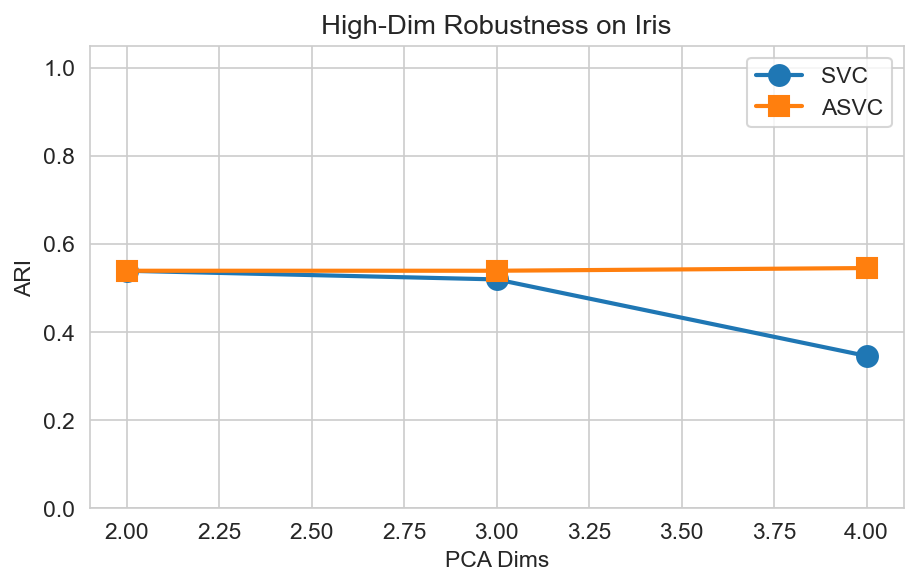
\includegraphics[width=\columnwidth]{fig/highdim.png}
\caption{High-dimensional robustness on Iris with varying PCA dimensions.}
\label{fig:highdim}
\end{figure}

\begin{figure}[t]
\centering
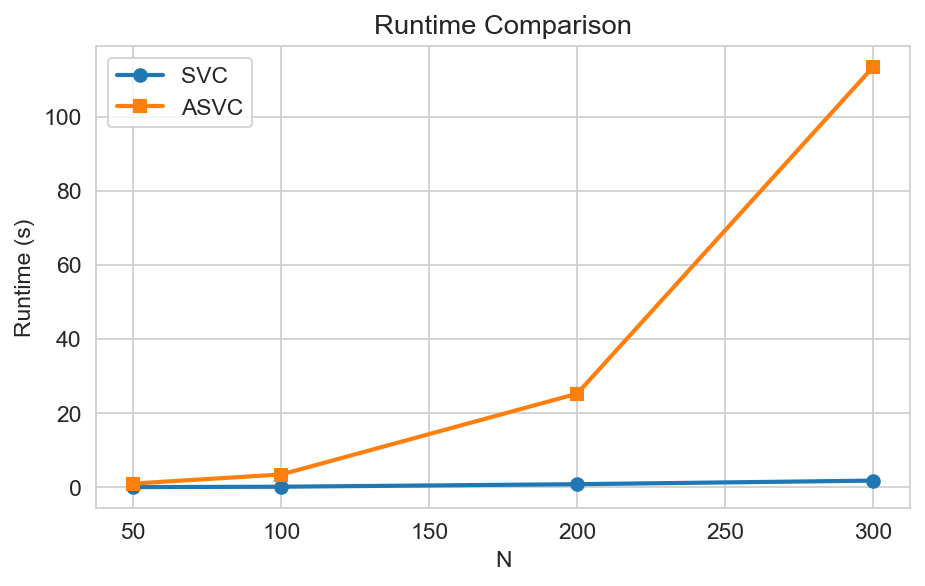
\includegraphics[width=\columnwidth]{fig/runtime.png}
\caption{Runtime comparison. ASVC incurs approximately 28$\times$ overhead from its two-phase search.}
\label{fig:runtime}
\end{figure}

\section{Conclusion}

We have presented Adaptive Support Vector Clustering (ASVC), which addresses the core practical limitation of original SVC in unsupervised scenarios---its ``cliff-like'' sensitivity to the kernel width $q$---through an automatic parameter selection mechanism. ASVC's innovations include: $k$-NN local-statistics-based $q$-range estimation, a two-phase parameter search strategy, and a dedicated continuous scoring function for SVC. Systematic experiments on six synthetic datasets demonstrate that: (1)~ASVC maintains non-trivial clustering performance across all datasets (minimum ARI~$\geq$~0.428), eliminating the risk of SVC's ``complete failure''; (2)~on datasets where SVC fails entirely, ASVC reverses ARI from 0 to 0.96--0.99; (3)~the VaryingBlobs experiment validates ASVC's density-independent clustering property. ASVC advances SVC from a ``laboratory tool'' requiring expert-guided parameter selection to a practical clustering method deployable independently in unsupervised settings.

\textbf{Code availability.} All experimental code, dataset generation scripts, and result reproduction workflows are open-sourced at \url{https://github.com/tuantuan-zi/ASVC}.
